\chapter{Introduction to succinct data structures}
\label{kap:kap1}

\section{Motivation}

In many applications, the amount of data is so significant that we optimise how much
storage these structures use. The field of \textit{succinct data structures focuses}
on representing data using as little space as possible while trying not to hurt the
runtime of methods that these data structures support. In this field, data structures
for many varied problems have been already devised. While many of these give some solid
theoretical bounds on the used space, others look into real-world space usage and
performance. The common disadvantage is that these structures are often more complicated
than their space non-efficient alternatives as they contain concepts and computation
patterns that are slower on modern computers.

The primary use case of these structures comes in two flavours. The first case is
that we have a lot of data and are trying to implement some useful methods working
with them. The problem we face with regular data structures supporting these
operations is that they may not even fit into our entire physical memory. The
second use case may be that even if we have an amount of data that could fit
into our computer, we instead use a succinct representation. This may enable us
to store the data in a faster type of memory (e.g. fast RAM instead of the
slower disk). Thus, even if we use more advanced concepts, the overall runtime
may decrease.

The work in this field turns focus more and more towards the dynamic succinct
data structures. These are structures where the underlying data may change after
constructing the structure. However, in this work, we will only consider static
succinct data structures. These are the ones where we get the data, then construct
the succinct data structure and then only support methods that do not alter the
underlying data in any way.

\section{FM-index}

One particularly useful succinct data structure is \textit{FM-index} proposed by Ferragina
and Manzini\cite{ferragina2000opportunistic}. It found a heavy use in the field of
Bioinformatics. Let us consider the problem of representing a text $T$ that we want to
store effectively. We can represent the text as a sequence over some alphabet $\Sigma$.
On top of that, we want to efficiently count or locate occurrences of pattern $P$
in this text. FM-index can find the pattern in time complexity $\mathcal{O}(|P|)$
after preprocessing the original text. On top of this, the resulting
space used by FM-index is for many applications smaller than the space used for the
original text $T$. This makes FM-index particularly useful for searching in very long sequences
of DNA where FM-index many times takes just 30-40\% of the space needed for the representation
of original DNA sequence. We shall now look at how the FM-index is obtained for the text $T$.
For simplicity, we assume that text $T$ contains a special character \$ located at the end
that is contained in $\Sigma$ and lexicographically smallest.

\subsection{Burrows-Wheeler transformation}

\textit{Burrows-Wheeler transformation} (BWT) lies at the heart of the FM-index, so we show
how it is constructed. We consider the sequence $S$ of symbols over
some alphabet $\Sigma$. Now we take all the cyclical rotations $S_1, S_2, \ldots S_n$ of the
sequence $S$ and put them into the rows of table sorted by their lexicographical order as
seen in Fig. \ref{obr:BWT}. We name the sequence created by the concatenation of symbols
in first and last column $F$ and $L$ respectively. Last column $L$ is what we also call
the BWT transformation of $S$. Computing BWT is useful step before compressing
the text as this operation is reversible and most of the time $S_{BWT}$ is more compressible
than $S$. We will show how to get $S$ from $S_{BWT}$ in the next section. The sequence $F$ can
be obtained from $L$ just by sorting all the characters in $S_{BWT}$. Note that $F$ has some
nice properties. It consists of of runs of symbols that are sorted according to the lexicographical
ordering of alphabet symbols. We will use the helper sequence $Count$ where $Count[c]$ is
number of occurrences of $c\in\Sigma$ in $S$. Although $Count$ uniquely represents $F$ we will
find also useful array $CountSmaller$ where $CountSmaller[c]$ is a total number of occurrences
of symbols smaller than $c$.

\begin{figure}
	\centerline{
	\begin{tabular}{l|c|ccccc|c|}
	\cline{2-8}
	  & \multicolumn{1}{l|}{\textbf{F}}    & \multicolumn{5}{l|}{}                                                                                                                                                                                                         & \multicolumn{1}{l|}{\textbf{L}}    \\ \cline{2-8} 
	1 & {\color[HTML]{333333} \textbf{\$}} & \multicolumn{1}{c|}{{\color[HTML]{C0C0C0} b}}  & \multicolumn{1}{c|}{{\color[HTML]{C0C0C0} a}}  & \multicolumn{1}{c|}{{\color[HTML]{C0C0C0} n}}  & \multicolumn{1}{c|}{{\color[HTML]{C0C0C0} a}}  & {\color[HTML]{C0C0C0} n}  & {\color[HTML]{000000} \textbf{a}}  \\ \cline{2-8} 
	2 & {\color[HTML]{333333} \textbf{a}}  & \multicolumn{1}{c|}{{\color[HTML]{C0C0C0} \$}} & \multicolumn{1}{c|}{{\color[HTML]{C0C0C0} b}}  & \multicolumn{1}{c|}{{\color[HTML]{C0C0C0} a}}  & \multicolumn{1}{c|}{{\color[HTML]{C0C0C0} n}}  & {\color[HTML]{C0C0C0} a}  & {\color[HTML]{000000} \textbf{n}}  \\ \cline{2-8} 
	3 & {\color[HTML]{333333} \textbf{a}}  & \multicolumn{1}{c|}{{\color[HTML]{C0C0C0} n}}  & \multicolumn{1}{c|}{{\color[HTML]{C0C0C0} a}}  & \multicolumn{1}{c|}{{\color[HTML]{C0C0C0} \$}} & \multicolumn{1}{c|}{{\color[HTML]{C0C0C0} b}}  & {\color[HTML]{C0C0C0} a}  & {\color[HTML]{000000} \textbf{n}}  \\ \cline{2-8} 
	4 & {\color[HTML]{333333} \textbf{a}}  & \multicolumn{1}{c|}{{\color[HTML]{C0C0C0} n}}  & \multicolumn{1}{c|}{{\color[HTML]{C0C0C0} a}}  & \multicolumn{1}{c|}{{\color[HTML]{C0C0C0} n}}  & \multicolumn{1}{c|}{{\color[HTML]{C0C0C0} a}}  & {\color[HTML]{C0C0C0} \$} & {\color[HTML]{000000} \textbf{b}}  \\ \cline{2-8} 
	5 & {\color[HTML]{333333} \textbf{b}}  & \multicolumn{1}{c|}{{\color[HTML]{C0C0C0} a}}  & \multicolumn{1}{c|}{{\color[HTML]{C0C0C0} n}}  & \multicolumn{1}{c|}{{\color[HTML]{C0C0C0} a}}  & \multicolumn{1}{c|}{{\color[HTML]{C0C0C0} n}}  & {\color[HTML]{C0C0C0} a}  & {\color[HTML]{000000} \textbf{\$}} \\ \cline{2-8} 
	6 & {\color[HTML]{333333} \textbf{n}}  & \multicolumn{1}{c|}{{\color[HTML]{C0C0C0} a}}  & \multicolumn{1}{c|}{{\color[HTML]{C0C0C0} \$}} & \multicolumn{1}{c|}{{\color[HTML]{C0C0C0} b}}  & \multicolumn{1}{c|}{{\color[HTML]{C0C0C0} a}}  & {\color[HTML]{C0C0C0} n}  & {\color[HTML]{000000} \textbf{a}}  \\ \cline{2-8} 
	7 & {\color[HTML]{333333} \textbf{n}}  & \multicolumn{1}{c|}{{\color[HTML]{C0C0C0} a}}  & \multicolumn{1}{c|}{{\color[HTML]{C0C0C0} n}}  & \multicolumn{1}{c|}{{\color[HTML]{C0C0C0} a}}  & \multicolumn{1}{c|}{{\color[HTML]{C0C0C0} \$}} & {\color[HTML]{C0C0C0} b}  & {\color[HTML]{000000} \textbf{a}}  \\ \cline{2-8} 
	\end{tabular}
	}
	\caption[TODO]{All the cyclic rotations of sequence $S = banana\$$. BWT is a last column. Note that we are not storing information about data with grey color.}
	\label{obr:BWT}
\end{figure}

\subsection{LF-mapping}

Useful information, that will be used in the future is something what we call \textit{LF-mapping}.
This is a mapping that for a symbol on $i$-th row in $L$, gives us a corresponding row in $F$
where this exact symbol is located. This is quite easy to obtain if the underlying sequence $S$
does not contain duplicate symbols. Now all the runs in $F$ vector will be of length 1.
To find $LF(i)$, we will simply look what is the $i$-th symbol in $L$. The run of
symbol $L[i]$ begins on the index $CountSmaller[L[i]] + 1$ so the formula can be written as:

$$LF(i) = CountSmaller[L[i]] + 1$$.

If we drop our requirement that every symbol is contained in the sequence $S$ at most once
we are seemingly in a more complicated situation. The problem may seem that even
though we still easily identify the beginning of the run of $L[i]$, we do not
know which occurrence of symbol $L[i]$ corresponds to occurrence of $L[i]$ in $i$-th row.
Helpful property is that $i$-th occurrence of symbol $c$ in $L$ corresponds to the
$i$-th occurrence of $c$ in $F$. So we can just change the final formula to

				$$LF(i) = CountSmaller[L[i]] + rank_{L[i]}(i)$$

where $rank_c(i)$ represents the number of occurences of $c$ up to $i$-th index inclusive.

\subsection{Reverse Burrows-Wheeler transformation}

We already stated that the BWT is reversible. So from the $T_{BWT}$ we are able to reconstruct
$T$. We do it by first obtaining $F$ from $T_{BWT}$. Now, we will iteratively reconstruct $S$
from the end to the beginning. First, we look to the first position in $F$ where last symbol
of $S$ - \$ - is located. We see what symbol is preceding \$ in $S$. This is a symbol
$L[1]$. Using the LF-mapping we find where $L[1]$ is located in $F$ and then repeat this process
until $L[i]$ is equal to \$.

\subsection{Supported methods}

As we already stated, FM-index is used for searching in the preprocessed text.
It does this using three methods:

\begin{itemize}
\item $locate(P)$ returns all positions of pattern $P$ in text $T$
\item $count(P)$ counts the number of occurences of $P$ in text $T$
\item $extract(i, j)$ returns the subsequence $T[i..j]$
\end{itemize}

The reason that the $extract$ method is useful and non-trivial is that FM-index
does not store the original sequence $T$ - at least not in an easily readable form.

%TODO: Implementacia operacii

\section{Storing elements of non-uniform size}

When trying to optimise the space used, it may be beneficial to use variable-length
code for symbols such as Huffman code. The problem is that even storing elements
like this in the array is problematic. With the variable-length elements, we do not
have a trivial and fast way to tell where $i$-th element is located. Even though
there are many solutions, one of them that is used quite often is storing these
elements one after another in memory. Then alongside this raw sequence of bits,
we have another helper bit-vector of the same size. This bit vector has ones on
places where the representation of the element starts and ones on the other places.

In the first row, we can see the elements stacked one after another. These elements
are of variable size as they need 4, 4, 2, 1 and 2 bits respectively to be stored.
Under the elements from the main vector, there is another helper bit-vector. Every
symbol of one in the helper vector corresponds to one element in the main vector
and is positioned in a place where the element's representation begins in the main vector.

To find the beginning of $i$-th element, we now transformed this task to find the
$i$-th one in the helper array. We shall call this method $select_c(i)$ and later
see how it can be implemented efficiently.

\begin{figure}
	\centerline{
	\begin{tabular}{l|l|l|l|l|l|l|l|l|l|l|}
	\cline{2-11}
	\textbf{Raw binary representation} & 1          & 1 & 0 & 1 & 1          & 1 & 1          & 0 & 1 & 0          \\ \cline{2-11} 
	\textbf{Helper bit array}          & \textbf{1} & 0 & 0 & 0 & \textbf{1} & 0 & \textbf{1} & 0 & 0 & \textbf{1} \\ \cline{2-11} 
	\end{tabular}
	}
	\caption[TODO]{Raw binary representation of elements 1101, 11, 101 and 0 stored one after another.
	Note the helper bit array that is of the same size with ones on the positions where new element begins.}
	\label{obr:VariableSizedElements}
\end{figure}

\section{Space efficiency}

There are many ways to measure the space efficiency of a data structure. From the
practical point of view, we may be interested in the memory usage by the data
structure on actual data that the structure could encounter in our use case. However,
many succinct data structures are trying to achieve some upper bounds and express
the used space in terms of the information contained in the data. There are many
models how to measure the information contained in sequences of characters. One
of the most commonly used models in the field of succinct data structures, yet still
quite simple, is entropy or more specifically zeroth-order entropy:

$$H(S)=\sum_{c\in\Sigma} \frac{n_c}{n} \lg \frac{n}{n_c}$$.

In many scenarios, where succinct data structures are used, the stored sequence
is compressible using the sole fact that some symbols have a bigger frequency than others.

\section{Wavelet tree}
\label{section:WaweletTree}

We shall assume for a moment that we have a bit-vector implementation supporting
access, rank and select methods. We show how this may be used to create
a more general version of this implementation representing sequence over arbitrary
alphabet still supporting access, rank and select queries in reasonable time complexity.

\textit{Wavelet tree} uses a divide-and-conquer approach. It takes the sequence $S$ of
length $n$ over some alphabet $\Sigma$ and recursively splits the alphabet into
two subsets creating a hierarchical partitioning of an alphabet. In the top node
of the tree, it splits the alphabet $\Sigma$ into two subsets of the roughly same
size $\Sigma_1, \Sigma_2$. It then stores a bit vector $B$ of size $n$ in this node
where
\[
    B[i]= 
\begin{cases}
    0,& \text{if } S[i]\in \Sigma_1\\
    1,              & \text{otherwise}
\end{cases}
\]

It then recursively applies the same idea on a subsequence of $S$ that is created
from $S$ by taking just symbols of $\Sigma_1$ ($\Sigma_2$) to create the left (right)
child nodes.

\begin{figure}
	\centerline{
		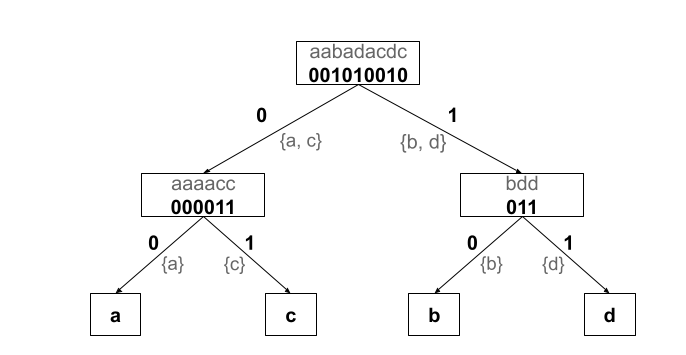
\includegraphics[width=0.9\textwidth, height=0.3\textheight]{images/wavelet_tree}
	}
	\caption[TODO]{Wavelet tree representation of text $S=aabadacdc$. We can see how the
	recursive partitioning of the alphabet works. In every node, we also show the
	subsequence represented (grey text) in the subtree of the node. The stored data can be
	recognized as they are in bold and black.
	}
	\label{obr:WaveletTreeExample}
	% based on https://simongog.github.io/assets/data/sdsl-slides/tutorial#23
	% source at https://docs.google.com/drawings/d/1cJyda3bdTluajr3iXu1x1iL5HF0JPZqAHw6jwct9KLI/edit
\end{figure}

Rank and select methods on the original sequence can be implemented using the tree
traversal and rank/select methods on the individual bit-vectors. Another modification
studied by M{\"a}kinen et. al.\cite{makinen2005succinct} is to shape the binary tree in a way that a Huffman
tree of the sequence symbols is shaped. Huffman tree is a tree constructed in the
process of creating Huffman encoding of the characters contained in the sequence.